\documentclass[a4paper, 10pt, titlepage]{scrreprt}

\linespread{1.5}					%Zeilenabstand 1,5mm
\parindent0cm						%Absatz wird nicht reingerückt

\usepackage[utf8]{inputenc}
\usepackage{graphicx}				%Zum Einbinden von externen Grafiken (jpeg,pdf)
\usepackage{a4wide}					%Ausnutzen der ganzen Blattbreite
\usepackage{fancyhdr} 				%Package für Kopf- und Fusszeile
\usepackage[ngerman]{babel}		%Rechtschreibung
\usepackage{hyperref}				%Einfügen von Weblinks
\usepackage{amsmath}				%Paket für mathematische Formeln
\usepackage{amsfonts}				%zusätzliche mathematische Zeichen
\usepackage{amssymb}				%zusätzliche mathematische Symbole
\usepackage[labelfont=bf]{caption}  %"Abbildung" fett geschrieben
\usepackage{subfigure} %Bilder da plazieren wo sie auch im Latex-Code stehen
\usepackage{graphicx}
\usepackage{eso-pic,picture}
\usepackage[absolute]{textpos}
\usepackage{hyphenat}
\usepackage[onehalfspacing]{setspace}
\usepackage{multirow}
\usepackage{array}
\usepackage{caption}
\usepackage{url}
\usepackage{chngcntr}
\usepackage{tikz}
\counterwithin{figure}{section}
\usepackage[a4paper, left=3.5cm, right=2.5cm, top=2.0cm, bottom=2.0cm,footskip=1.5cm, includeheadfoot] {geometry}  % manuelles Seitenlayout
\usepackage{bibgerm}        % Einfügen des Literaturverzeichnisses
\usepackage{eurosym}        % Einfügen des € Zeichens
%\usepackage{lscape}        % Text einer Seite wird im quer dargestellt
%\usepackage[a4paper]{geometry}                     % Querformat einer Seite
\usepackage{pdfpages}       % Einfügen von ganzen PDF-Seiten
\usepackage{array}

%================================================================================

%% definieren einer neuen Tabelle mit automatischen Umbruch
\newcolumntype{C}[1]{>{\centering\arraybackslash}m{#1}}%m-vertikal zentriert, b bottom, p top; allg: zur Definition einer festen Spaltenbreite
\newcolumntype{L}[1]{>{\raggedright\arraybackslash}p{#1}} % linksbündig mit Breitenangabe


%================================================================================

%Kopfzeile
%--------------------------------------------------------------------------------%\fancyhf{} %alle Kopf- und Fußzeilenfelder bereinigen
%\pagestyle{fancy} %eigener Seitenstil

%Kopfzeile links bzw. innen
%\fancyhead[L]{Michael Winzer}
%Kopfzeile mittig
%\fancyhead[C]{D-Nr./2014}
%\facnyhead[R]{\chaptermark}
%\renewcommand{\headrulewidth}{0.5pt}				%obere Linie

%Fußzeile
%--------------------------------------------------------------------------------
%\fancyfoot[R]{\thepage} 							%Seitennummer
%\fancyfoot[L]{\nouppercase{\leftmark}}							%Kapitelbezeichnung Position
%\renewcommand{\chaptermark}[1]{\markboth{\thechapter.~\chaptername: #1}{}}	%Kapitelbezeichnung 



%--------------------------------------------------------------------------------


\begin{document}


%Titelseite
%--------------------------------------------------------------------------------
\begin{titlepage}
\thispagestyle{empty} 		%Keine Kopf- und Fusszeilen, keine Seitenzahl
\linespread{1.0}

\begin{figure}

\includegraphics[scale=0.3]{images/HTW-Logo}
\end{figure}


\hrule
\vspace{0.2 cm}
\textbf{Fakultät Maschinenbau/Verfahrenstechnik,}
\vspace{0.1 cm}
\hrule
\vspace{0.2 cm}
Fahrzeugtechnik 



\begin{flushleft}
\vspace{8 cm}
\huge\textbf{Konstruktive Weiterentwicklung eines modularen Batteriespeichers  in  
20‘-Containerbauweise für PV - Hybridkraftwerke}\\ [0.5 cm]
\Large{Untertitel bzw. nähere Beschreibung des Themas oder der Aufgabenstellung}\\ [1.5 cm]
\Large{Dresden, DATUM}
\end{flushleft}

\pagebreak 

\thispagestyle{empty} 		%Keine Kopf- und Fusszeilen, keine Seitenzahl

\begin{figure}

\includegraphics[scale=0.3]{images/HTW-Logo}
\end{figure}

\hrule
\vspace{0.2 cm}
\textbf{Fakultät Maschinenbau/Verfahrenstechnik,} 
\vspace{0.1 cm}
\hrule
\vspace{0.2 cm}
Studiengang Fahrzeugtechnik

\begin{center}
\vspace{2 cm}
\huge\textbf{ART DER ARBEIT}
\huge\textbf{(DIPLOMARBEIT)}
\vspace{2 cm}
\end{center}



\begin{tabular}{lL{6,5cm}}
\Large\textbf{Thema:} & \Large{Konstruktive Weiterentwicklung eines modularen Batteriespeichers in 20‘-Containerbauweise für PV - Hybridkraftwerke}\\
\Large\textbf{Bearbeiter:} & \Large{Michael Winzer}\\
\Large\textbf{Matrikelnummer:} & \Large{28563}\\
\Large\textbf{Bearbeitungszeitraum:} & \Large{TT.MM.JJ bis TT.MM.JJ}\\
\Large\textbf{Ort, Datum der Abgabe:} & \Large{Dresden, DATUM}\\
\Large\textbf{Nummer:} & \Large{XYZ}\\
\Large\textbf{Betreuer:} & \Large{Dipl. Ing. Lars Fallant}\\
\Large\textbf{Verantw. Hochschullehrer:} \hspace{1 cm} & \Large{Name des Hochschullehrers}\\
\vspace{1 cm}\\
\large{Textseiten:} & \large{xx}\\
\large{Anlagen:} & \large{yy}\\
\large{Anhänge:} & \large{zz}\\
\end{tabular}


\end{titlepage}
%
\linespread{1.5}

%Aufgabenstellung
%---------------------------------------------------------------------------------
\fancyhf{}

\thispagestyle{fancy}
\fancyhead[L]{Michael Winzer}
%Kopfzeile mittig
\fancyhead[C]{D-Nr./2014}
\fancyhead[R]{HTW-Dresden}
%\renewcommand{\headrulewidth}{0.5pt}
\Large\textbf{Aufgabenstellung}\\ 

Hier wird eine Kopie bzw. für das Bibliotheksexemplar das Original der ausgereichten Aufgabenstellung eingeordnet.

\pagebreak 




%Hauptteil
%---------------------------------------------------------------------------------
%Kapitel sind für eine bessere Übersicht in eigenen Dateien und werden hier aufgerufen:

\chapter*{Sperrvermerk}\thispagestyle{fancy}\markboth{Sperrvermerk}{1}
\addcontentsline{toc}{chapter}{Sperrvermerk}

Diese Praktikumsbericht enthält vertrauliche Informationen, die der Geheimhaltung unterliegen. Sie dürfen nur für die interne Verwendung und zur Kontrolle durch den verantwortlichen Hochschullehrer genutzt werden. Eine, auch nur teilweise, Veröffentlichung der Belegarbeit darf nur mit Zustimmung der BELECTRIC GmbH, Zweigstelle Dresden, Industriestraße 65, 01129 Dresden erfolgen.
\\ 
\\
\\
{\LARGE Dresden, DATUM}\\



%Kopfzeile
%-------------------------------------------------------------------------------- \fancyhf{} %alle Kopf- und Fußzeilenfelder bereinigen
\pagestyle{fancy} %eigener Seitenstil

%Kopfzeile links bzw. innen
\fancyhead[L]{Michael Winzer}
%Kopfzeile mittig
\fancyhead[C]{D-Nr./2014}
%\facnyhead[R]{\chaptermark}
\renewcommand{\headrulewidth}{0.5pt}				%obere Linie

%Fußzeile
%--------------------------------------------------------------------------------
\fancyfoot[R]{\thepage} 							%Seitennummer
\fancyfoot[L]{\nouppercase{\leftmark}}							%Kapitelbezeichnung Position
\renewcommand{\chaptermark}[1]{\markboth{\thechapter.~\chaptername: #1}{}}	%Kapitelbezeichnung 

\setcounter{page}{1}
\pagenumbering{Roman}
%Inhaltsverzeichnis plotten
%---------------------------------------------------------------------------------
\addtocontents{toc}{\protect\thispagestyle{fancy}}
\thispagestyle{fancy}
\tableofcontents
\thispagestyle{fancy}
% Abkürzungsverzeichnis
%---------------------------------------------------------------------------------

\chapter*{Abkürzungsverzeichnis}\thispagestyle{fancy}\markboth{Abkürzungsverzeichnis}{Abkürzungsverzeichnis}
\addcontentsline{toc}{chapter}{Abkürzungsverzeichnis}

\begin{tabbing}
\ \= \textbf{Abkürzung} \hspace{0.5cm} \= \textbf{Beschreibung} \kill
\\

\> BMS \>   Batterie-Management-System\\
\> EBU \>   Energy Buffer Unit\\
\> B\&R \>		Bernecker + Rainer Industrie-Elektronik\\
\> ST \>   Strukturierter Text\\
\> SQL \>   Structured Query Language\\
\> HTML \>  HyperText Markup Language \\
\> CSS \>   Cascading Style Sheets\\
\> PHP \>   Hypertext Preprocessor\\
\> CSV \>   Comma-separated values\\
\> JSON \>  JavaScript Object Notation\\
\> FTP \>   File Transfer Protocol\\



\end{tabbing}

% Symbolverzeichnis
%---------------------------------------------------------------------------------

\chapter*{Symbolverzeichnis}\thispagestyle{fancy}\markboth{Symbolverzeichnis}{Symbolverzeichnis}
\addcontentsline{toc}{chapter}{Symbolverzeichnis}

\section*{Formelzeichen}

\begin{tabbing}
\ \= \textbf{Symbol} \hspace{0.5cm} \= \textbf{Einheit} \hspace{1.5cm} \= \kill
\> $A$ \> $\mathrm{m^{2}}$ \> Fläche \\
\> $a$ \> $\mathrm{MPa}$ \> Kohäsionsdruck \\
\end{tabbing}

\section*{Griechische Symbole}

\begin{tabbing}
\ \= \textbf{Symbol} \hspace{0.5cm} \= \textbf{Einheit} \hspace{1.5cm} \= \kill
\> $\alpha$ \> $\mathrm{W\,/\,(m^{2} \cdot K)}$ \> Wärmeübergangskoeffizient\\
\> $\gamma$ \> - \> Aktivitätskoeffizient für die Flüssigphase \\
\end{tabbing}
% Abbildungsverzeichnis
%---------------------------------------------------------------------------------
\setcounter{lofdepth}{-1}
\listoffigures
\setcounter{lofdepth}{-1}
% Tabellenverzeichnis
%---------------------------------------------------------------------------------

\listoftables
\addcontentsline{toc}{chapter}{Tabellenverzeichnis}{\thispagestyle{fancy}}

\setcounter{page}{1}
\pagenumbering{arabic}
\chapter{Einleitung}\thispagestyle{fancy}

\Large {Die Firma Belectric GmbH wurde im 2001 gegr�ndet und hat sein Standort im Kolitzheim. Seit dem hat �ber 1,5 GWp Solarleistung weltweit installiert. Sie wurde somit eine Weltmarktf�hrer in den Bereich Installation von Freifl�chensolarkraftwerken. Es werden neue und innovative Technologien bei der Installation umgesetzt. Weltweit sind �ber 1600 besch�ftigte Menschen, die in Bereichen von Wartung und Anlagebau bis zu Forschen und Entwickeln beim Belectric arbeiten. \\
Die Firma Adensis GmbH, mit dem Standort im Dresden, geh�rt zu den Entwicklungs- und Forschungsgruppen der Belectric GmbH. Sie wurde im 2006 gegr�ndet und seit dem betreibt ein Forschungszentrum f�r den Gebiet Photovoltaik. �ber 70 Mitarbeitern sind in den Bereichen Elektrotechnik, Maschinenbau, Physik und Chemie angestellt. Einen gr��eren Teil der Mitarbeiter bilden Studenten und ehemalige Studenten.  Zu den Aufgabenfeldern der Adensis GmbH geh�rt Durchf�hren von Testen und Analysen, Entwicklung neuer Technologien und Produkte sowie Kraftwerksbau. \\
Meine 20-Wochige Praktikum wurde in den Abteilung Kraftwerkstechnik der Firma Adensis absolviert. Das Pflichtpraktikum war auf zwei Hauptthemen geteilt. Im Oktober habe ich mich mit einen Batterie-Management-System, der im Adensis entwickelt war,  besch�ftigt. Meine Aufgabe war einen Algorithmus f�r die B\&R Steuerung entwickeln sollen. Ab November war ich mit Visualisierung von gesendeten Daten aus einer Kraftwerksanlage besch�ftigt. Das soll mittels einer Website, mit jeweiligen Grafischen Mitteln realisiert werden.}

\vspace{2cm}

\begin{figure}[htbp]
  \centering
     
\includegraphics[width=0.6\textwidth]{images/Belectric-Logo.png}
  \caption{Logo Belectric}
  \label{fig:Logo Belectric}
\end{figure}

\vspace{2cm}

\begin{figure}[htbp]
  \centering
     
\includegraphics[width=0.6\textwidth]{images/adensis_logo.jpg}
  \caption{Logo Adensis}
  \label{fig:Logo Adensis}
\end{figure}

\chapter{Grundlagen}\thispagestyle{fancy}

\section{Allgemeines}
Allgemein orientieren sich Aufbau und Gestaltung der Diplomarbeit an den Normen zur Gestaltung wissenschaftlicher Arbeiten, siehe DIN 1421, 1422, 1502, 5008.
Die Diplomarbeit ist auf weißem Papier im Format A4 entsprechend den Richtlinien zur Textverarbeitung (DIN 5008, Duden) zu verfassen und zu binden.
Beleg- und Diplomarbeiten sind wissenschaftlich technische Dokumentationen, die allgemeinen Anforderungen bezüglich Struktur und Form entsprechen müssen. Sie sollen sich durch Klarheit im Ausdruck, guten Stil und einwandfreie Orthografie auszeichnen. Formulierungen sind sorgfältig zu wählen. Das betrifft auch die Verwendung fremdsprachiger Begriffe.
Die Arbeit ist logisch zu gliedern.
Der Schreibende soll einen anspruchsvollen wissenschaftlich-technischen Inhalt verständlich vermitteln. Dazu ist es erforderlich, sich immer wieder in die Position des Lesers zu versetzen und die Darstellung in dieser Hinsicht zu hinterfragen.
Das Bild, d. h. Prinzipskizze, Diagramm, Foto, Flussdiagramm, Tabelle etc., ist die „Sprache des Ingenieurs“ und sollte langen Erklärungen vorgezogen werden.
Ergebnisse müssen rückverfolgbar sein. Dazu sind die angewandten Methoden, Annahmen, Randbedingungen, experimentellen Einrichtungen und Programme sowie relevante Zwischenergebnisse zu nennen und in einem angemessenen Umfang zu erläutern.
Auch Berechnungen sind so zu dokumentieren, dass der Gutachter ihre Richtigkeit  überprüfen kann.
Die Darstellung sollte sich auf das Wesentliche konzentrieren und frei von allgemein bekannten Abhandlungen und „Füllstoff“ sein, die nur vom Thema ablenken und den „roten Faden“ verlieren lassen.
Der Arbeit ist eine schriftliche Erklärung beizufügen, dass sie selbständig angefertigt wurde und keine anderen als die angegebenen Unterlagen verwendet wurden.\\
Der Textteil der Arbeit besteht aus:
\begin{itemize}
\item Einleitung
\item Zielstellung
\item Lösungsweg
\item Hauptteil mit Unterabschnitten
\end{itemize}

\section{Einleitung}
Die Einleitung beschreibt den Aufbau der Arbeit, die Motive zu Ihrer Erstellung, die wissenschaftliche Herangehensweise an die Problemstellung sowie formale technische und ggf. rechtliche Rahmenbedingungen.

\section{Bindung}
Die Arbeit ist an der Professur in zweifacher Ausfertigung in gebundener Form (Ringbindung, feste Bindung), ausgedruckt auf weißem Papier (80 $g/m^{2}$), Format DIN A4, abzugeben. Die eigentlichen Seiten sind bei Ringbindung mit zwei leeren Deckblättern ($>$ 120 $g/m^{2}$) zu umschließen.\\
Für Diplom-, Master- und Bachelorarbeiten ist eine feste Bindung vorgeschrieben. Bitte die Exemplare beschriften (Rücken [Beschriftung 2 cm ab unterem Rand beginnen] und Deckel) mit DA Nr., Name, Vorname. \\
Muster hierzu können im Zweifelsfall in der Professur eingesehen werden.

\section{Elektronische Form}
Der ausgedruckten und gebundenen Arbeit ist eine CD/ DVD in einer Tasche auf der letzten Seite der Arbeit beizulegen. \\
Darauf ist die Arbeit als Datei, z. B. Word-Datei, alle erstellten elektronischen Modelle, Simulationen, Programme, Zeichnungen, Fotos, Vorlagen, Rechnungen usw. jeweils in weiter bearbeitbaren Formaten (SolidWorks, AutoCAD, Corel, Cosmos, Fluent, ComSol, jpg, bmp, MathCAD, ...) und recherchiertes Material, das Ihnen in elektronischer Form vorliegt (Zeitschriftenartikel, Scans, Auszüge aus Büchern, e-books, ...), mit abzulegen. \\
Sämtliche Dateien sind unverschlüsselt abzuspeichern.

\section{Formatierung}
\subsection{Allgemeines}
Alle Formatvorlagen und Seitenformate sind dieser Vorlage zu entnehmen. Fertigen Sie sich eine Kopie dieser Datei an. Benennen Sie diese dann um und löschen vorsichtig, Absatz für Absatz die Texte. Behalten Sie die sich automatisch aktualisierenden Verzeichnisse und Nummerierungen bei. Das vereinfacht den Einstieg in die Arbeit.

\subsection{Abkürzungen und physikalische Größen}
Sämtliche Abkürzungen sind mit ihrer ersten Verwendung einzuführen und entsprechend im Abkürzungsverzeichnis aufzunehmen. \\
Die Auflistung im Abkürzungsverzeichnis gilt auch für ``z. B'' oder ``etc.''. Abkürzungen, die für mehrere einzelne Wörter stehen. Mehrere einzelne Wörter wie ``z. B.'' oder ``u. a.'' sind auch in der Abkürzung durch ein Leerzeichen (empfohlen wird zur Vermeidung des ``Auseinanderziehens'' die Verwendung von $<$Backslash$>$ $<$Komma$>$ als Befehl für eine halbe Leerzeile) getrennt.\\
Genauso ist bei der Darstellung von Betrag und Einheit zu verfahren. (Beispiele: $5,67\, W/(m^{2}K^{4})$, $9,6 MJ/kg$, $12,0 \cdot 10^{-6}\,1/K$, $100\,^{\circ}\mathrm{C}$, $26\,\%$, jedoch: $90\,^{\circ}$).\\
Physikalische Größen sind in Maßeinheiten des internationalen Einheitensystems (SI) anzugeben, d. h. bei Verwendung historischer oder anglo-amerikanischer Quellen mit Nicht-SI-Einheiten (z B. atü, $mmWS$, $Torr$, $psi$, $^{\circ}F$, $kcal$, $PS$, $ft$, ...) entsprechend umzurechnen. Die Umrechnung ist in jedem Fall in der Arbeit zu dokumentieren.

\subsection{Absätze und Überschriften}
Unter Hauptüberschriften der Ebene 1, die mit Überschriften der Ebene 2 weiter unterteilt werden, wird kein Text eingefügt. Es sind entsprechende ``Einleitungs-Unterkapitel'' einzufügen.
Die maximale Gliederungstiefe für Diplomarbeiten beträgt 3 Ebenen. Entsprechend enthält das Inhaltsverzeichnis nur die Überschriften der Ebene 1 – 3.\\
Es ist der Blocksatz zu verwenden.

\subsection{Schriftgröße und Zeilenabstand}
In den jeweiligen Formatvorlagen sind die Schriftgröße (mind. 11) und der Zeilenabstand (1,5) geregelt.

\section{Rechtschreibung und Grammatik}
Die studentische Arbeit ist in der Regel in deutscher Sprache und dabei nach den Regeln der neuen deutschen Rechtschreibung anzufertigen.

\section{Quellen und Zitate}
Es ist ein Quellenverzeichnis zu führen. Wörtlich zitiert wird in Anfüh- rungszeichen mit einem Quellenverweis. \\
Beispiele: \\
Nach Meinung vom VERFASSER wird ``… wie hier zu sehen, wörtlich zitiert''.\\
Enthält das Zitat bereits einen abschließenden Satz-Schluss-Punkt, wird nach der schließenden Klammer der Quellenangabe kein Punkt gesetzt. \\
Die drei Punkte (…) werden in Zitaten verwendet, um alle Auslassungen zu kennzeichnen. 
Auch hier liefert der VERFASSER mit der Forderung ``… den bedingungslosem Einsatz … der Punkte … bei Auslassungen'', ein gutes Beispiel. \\
Bei drei Punkten am Ende eines Zitates wird ``… dringend der Punkt nach der Quellenangabe gesetzt …''.\\
Die Abkürzungen ``f.'' und ``ff.'' stehen für die Folgeseite bzw. die Folgeseiten.
Verweise zu Quellen sind in eckigen Klammern auszuführen, wie beispielsweise nachstehend für die 37. BImSchV. \cite{BImSchV}

\section{Fussnoten}
Kurzworte (z. B. REA\footnote{REA: gebräuchliches Kurzwort für Rauchgasentschwefelungsanlage} ), fremdsprachige (z. B. Betula pendula\footnote{Betula pendula: lat. für Hänge-Birke} ) und fachgebietsfremde Fachbegriffe sowie Markennamen (z. B. PERSIL\footnote{PERSIL: Vollwaschmittel, eingetragene Marke der Henkel AG, Düsseldorf} ) sind auf der Seite der ersten Nennung mittels einer Fußnote zu erklären. 

\section{Abbildungen und Tabellen}
Platzieren Sie alle Abbildungen und deren Beschriftung in Tabellen ``ohne Rahmen'' (2 Zeilen und 1 Spalte, bei zwei Stück nebeneinander liegenden Bildern: 2 Zeilen und 2 Spalten). \\
Beschriften Sie alle Abbildungen mit Bildunterschrift und Tabellen mit Tabellenüberschrift. \\
\\

\begin{figure} [h]
\centering

\includegraphics[scale=0.6]{images/Abbildung1.png}
\caption{Logo Professur}
\end{figure}

Am Ende der Arbeit wird je ein entsprechendes Verzeichnis eingefügt. Abbildungen aus dem Anhang werden hier nicht aufgeführt. Zentrieren Sie Ihre Grafiken und Tabellen.
\\
\begin{table} [h]
\begin{center}
\caption{Tabellenübersicht}
\begin{tabular}{|c|c|c|}
\hline 
Spalte 1 & Spalte 2 & Spalte 3 \\
\hline
Text & Text & Text \\
\hline
 & & \\
\hline
\end{tabular}
\end{center}
\end{table}
\\

Quelltexte und große Grafiken (im Format einer Seite) sollten in den Anhang verschoben werden, es sei denn der Lesefluss wird dadurch erheblich gestört. Dies ist z. B. der Fall, wenn die Grafik einen Abschnitt zusammenfasst. 

\section{Formeln}
Verwendung Sie zur Darstellung der Formeln den Mathematikmodus von LaTex. Die Nummerierung der Formeln sollte vorhanden sein.\\

\begin{equation} 
\dot{Q}_{Strahl} = C_{1,2} \cdot A_{1} \cdot \left[\left(\frac{T_{1}}{100}\right)^{4} - \left(\frac{T_{2}}{100}\right)^{4}\right]
\end{equation} 

\section{Veröffentlichung}
Studentische Arbeiten sind als wissenschaftliche Arbeiten öffentlich zu- gänglich. Sollte die Arbeit vertrauliche Informationen enthalten, die nicht veröffentlicht werden können, so ist der Textteil zumindest so zu verfassen, dass wissenschaftlicher Hintergrund, Lösungsweg und grundsätzliche Aussagen vom Leser nachvollziehbar sind. Dies ist z. B. durch normierte Diagramme und Prinzipdarstellungen möglich. Vertrauliche Daten sind in diesem Fall in einem nicht öffentlichen Anlageteil beizufügen, der nur den Gutachtern zur Prüfung der Arbeit zugänglich ist. (aus \cite{Dokument})

\section{Kommentare am rechten Blattrand}
Alle Kommentare dieser Vorlage sind in der Endversion Ihrer Arbeit zu löschen.



\chapter{Betreuung des Studenten}\thispagestyle{fancy}

Eine Betreuung des Studenten ist insbesondere bei Diplomarbeiten unerlässlich. Um diese für beide Seiten möglichst effizient zu gestalten, ist es ratsam, folgende Punkte zu beachten:

\begin{itemize}
\item Vor jedem Gespräch ist ein Termin (telefonisch, E-Mail) zu vereinbaren. 
\item Die Fragen und Diskussionspunkte sind zuvor vom Studenten stichpunktartig schriftlich zu fixieren. Um Redundanzen zu vermeiden, ist es ratsam, auch die Ergebnisse zu notieren. 
\item Es sollte frühzeitig eine Gliederung erstellt werden, die mit dem Betreuer diskutiert werden kann. 
\end{itemize}

Die aktuell zu vergebenden Beleg- und Diplomarbeitsthemen können an der Professur erfragt werden (Dr.-Ing. Thomas Sander, 463 33097, thomas.sander@tu-dresden.de) und werden auf der \href{http://tu-dresden.de/die_tu_dresden/fakultaeten/fakultaet_maschinenwesen/iet/ew/beleg_da_arbeiten}{Homepage der Professur} publiziert.
\chapter{Zusammenfassung und Ausblick}\thispagestyle{fancy}

Die Arbeit wird durch eine Zusammenfassung und einen Ausblick abgeschlossen. Dieser bildet in diesem Sinne das Gegenstück zur Einleitung, d. h. hier werden die dort beschriebenen Ziele und der verwendete Weg kritisch beleuchtet.\\
Zum Schluss noch ein paar allgemeine Hinweise:

\begin{itemize}
\item \textbf{Legen Sie Wert auf den roten Faden!} Beschreiben Sie stets Ihren Weg durch das Thema so, dass er problemlos nachvollzogen werden kann. Die Einleitung bietet hier Raum für einen Überblick, sparen Sie nicht an einleitenden und zusammenfassenden Sätzen für Abschnitte der Ebene 1.
\item \textbf{Verdeutlichen Sie komplexe Zusammenhänge grafisch!} Ohne in Marketing-Icons zu verfallen, hilft oft eine einfache Grafik, um komplexe Zusammenhänge zu verdeutlichen. Nutzen Sie zur Visualisierung Ihrer Ausführungen Programme mit vielfältigen Möglichkeiten (z. B. Inkscape oder Excel). Verwenden Sie die Formen, Farben und Schattierungen dezent! 
\end{itemize}

\begin{figure}[h]
\centering
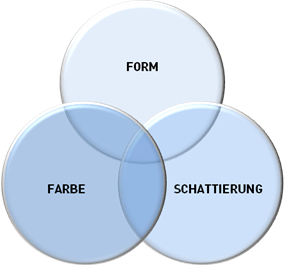
\includegraphics[scale=1.0]{images/Abbildung2.png}
\end{figure}

\begin{itemize}
\item \textbf{Vergessen Sie nicht Ihre Unterschrift unter die Eidesstattliche Erklärung!} Kontrollieren Sie sicherheitshalber jedes Exemplar vor der Abgabe! 
\item Kontrollieren Sie die \textbf{Vollständigkeit} der Exemplare! Achten Sie darauf, dass sich die Formatierung aufgrund von unterschiedlichen Druckern (Ihr Drucker und der Drucker im Copy-Shop) ändern kann. 
\item \textbf{Anzahl einzureichender identischer Exemplare:} zwei 
\end{itemize}
% Literaturverzeichnis
%---------------------------------------------------------------------------------
\bibliographystyle{unsrtdin}
\bibliography{Quellen}

 
% Indizes
%---------------------------------------------------------------------------------

\chapter*{Indizes}\thispagestyle{fancy}\markboth{Indizes}{Indizes}
\addcontentsline{toc}{chapter}{Indizes}

\begin{tabbing}
\ \=  \textbf{Symbol} \hspace{0.5cm} \= \textbf{Bedeutung} \kill
\> A \> Asche \\
\> AG \> Abgas \\
\> BS \> Brennstoff \\
\> BK \> Brennkammer \\
\> el \> elektrisch \\
\> FL \> Falschluft \\ 
\> KÜHL \> Kühlung \\
\> L \> Luft \\
\> REZI \> Rezirkulation \\
\> RG \> Rauchgas \\
\> th \> thermisch \\
\end{tabbing}
% Eidesstattliche Erklärung
%---------------------------------------------------------------------------------

\chapter*{Eidesstattliche Erklärung}\thispagestyle{fancy}\markboth{}{}
\addcontentsline{toc}{chapter}{Eidesstattliche Erklärung}

Hiermit versichere ich, \textit{Vorname und Name des Studenten}, die vorliegende Arbeit selbständig, ohne fremde Hilfe und ohne Benutzung anderer als der von mir angegebenen Quellen angefertigt zu haben. Alle aus fremden Quellen direkt oder indirekt übernommenen Gedanken sind als solche gekennzeichnet. \\
Die Arbeit wurde noch keiner Prüfungsbehörde in gleicher oder ähnlicher Form vorgelegt.\\
\\
Dresden, DATUM\\
\\

..............................\\
Vorname und Name des Studenten

\chapter*{Anhang}\thispagestyle{fancy}\markboth{Anhang}{}
\addcontentsline{toc}{chapter}{Anhang}


% Datenträger 
%---------------------------------------------------------------------------------

\chapter*{Datenträger}\thispagestyle{fancy}\markboth{}{}
\addcontentsline{toc}{chapter}{Datenträger}

Hier ggf. ist die CD oder DVD in einer geeigneten Folienhülle stabil zu befestigen.





\end{document}